%!TEX root = ../../dissertation.tex
%%%%%%%%%%%%%%%%%%%%%%%%%%%%%%%%%%%%%%%%%%%%%%%%%%%%%%%%%%%%%%%%%%%%%%%%%%%%%%%%
\subsection{Cross-Layer Information Exchange}
\label{c5:sec:crosslayerhinting}

The Internet has its historic roots deep in wired networks with a slim and well-defined network stack represented by the \gls{ISO}/\gls{OSI} or \gls{TCP}/gls{IP} model. These layers are isolated against each other. Only predefined information exchange points, or \gls{osiSAP}, at the layer borders allow for vertical communication. A typical wired Internet environment consists of either an Ethernet or other access technologies, e.g., \gls{DSL} or \gls{DOCSIS}, at the physical and link layers or \gls{PON} with \gls{TCP}/\gls{IP} following atop.

Application layer protocols often implicitly rely on the presence and characteristics of specific lower layer protocols. Through the layer isolation no application can precisely know or even control the current state of the lower layers. Nonetheless, they make assumptions on the composition and behavior of the lower layers and plan their work accordingly. 

But the access technology diversity has strongly increased through the advent of wireless technologies, and past behavioral patterns may not be applicable any more today. The protocols used for the radio transmissions behave very differently when compared to Ethernet and assumptions made by higher layers may not hold any more. Examples for this were given in the in the discussion of the stack's influences in Section~\ref{c5:sec:stack-influences}.

It would be very desirable for transport and application layer mechanisms to be able to understand this and cope with these effects. The term \textit{cross-layer interactions} or \textit{information exchange} subsumes these approaches. Specific information from one layer is made available to other interested layers and can even skip intermediate layers. Using cross-layer techniques many of the previously introduced layer influences can be diminished or neutralized altogether.

The next sections describe related mechanisms in the literature, classifications and then proceed to describe a new cross-layer approach that facilitates cross-layer information to the benefit of mobile streaming. The cross-layer work is based on a proposal for a FWF~\footnote{Fonds zur Förderung der wissenschaftlichen Forschung, \url{http://www.fwf.ac.at/}} stand-alone project submitted in October 2014 \todo{replace with actual date}. Thus, only initial ideas and planned future work is described.


\subsubsection{Related Cross-Layer Approaches and Classifications}

The idea of exchanging information between layers is not a particularly new one. Some specific ideas have been implemented a long time ago. The authors \cite{Raisinghani2004720} list a number of scenarios in which cross-layer information could be used and also talk about the type of information to be shared between layers.

One of the oldest and most well known cross-layer approaches is probably \gls{ECN}~\cite{rfc3168}. Here, the \gls{IP} layer of intermediate hops can signal the end nodes' \gls{TCP} layer that congestion is occurring and \gls{TCP} does not need to wait for implicit congestion signals, e.g., duplicate acknowledgments or timeouts. However, \gls{ECN} is disabled in almost every implementation as it lead to numerous problems and triggered bugs\footnote{\url{http://lkml.iu.edu//hypermail/linux/kernel/0009.1/0329.html}}. This is a risk that many cross-layer attempts may face.

A significant amount of publications is dealing with cross-layer information in wireless and mobile protocol stacks. A number of architectures have been proposed, e.g., \cite{raisinghani2004eclair, 1580937}, \cite{wang2003multi}, \cite{1200522}, and \cite{krishna2007cross}, but no actual solution seems to have been implemented in any of these.

While cross-layer typically implies a solely \textbf{vertical} exchange flow there can also be \textbf{horizontal} components present. \gls{DLEP}~\cite{ietf2013dlepdraft} is such an example of a \textbf{diagonal} flow, providing information of a lower layer of one entity to a higher layer at another node.
The \gls{DLEP}~\cite{ietf2013dlepdraft,6379143} protocol provides information available only to the (external) wireless modem or other interfaces to the routing entity of a node upon which it can act. Link characteristics such as bandwidth, latency, connection status, or information regarding neighbors can be requested.

Though, horizontal information flow is more than often an indication of \textbf{centralization} (also called \textbf{network-assisted} or \textbf{managed}) as apposed to purely vertical \textbf{distributed} approaches. Concerning network-assisted cross-layer exchange there are a number of approaches, that aim to integrate layer cooperation into the design of new mobile network infrastructures, including \cite{zarai2010seamless} and \cite{Piamrat20111066}. Generally, information is retrieved from the clients and collected at a central manager to be used in any policy decision like mobility and radio resource management.

Going back to purely distributed approaches, in \cite{hummel2010mobilitaet} the concept of mobility awareness is discussed. The goal is to predict motion and mobility based on available information and adapt the individual network layers to react accordingly. 

One of the easiest to implement uses of cross-layer information is the selection of the active network interface. Current mobile devices have a wide range of interfaces available, all with specific characteristics. The management architecture proposed in  \cite{Bonnin:2009:AMM:1503496.1503498} switches the currently used interface based on pre-configured profiles. Information from multiple layers is used to support the decision-making process.

To optimize unreliable video streaming in a WiFi network, the authors of \cite{1580941} create a control loop between the video encoder and the 802.11 \gls{MAC} layer to conduct WiFi rate control fitted to the output of the encoder. This is an example of a tight cross-layer control loop for one particular application, which has very likely adverse affects on other applications using this node.

The notion of cross-layer can also be applied to non-traditional network stacks. For example, the authors of \cite{4656786} present a cross-layer model for satellite communication stacks. They additionally distinguish between two general flavors of cross-layer architectures, one with \textbf{direct} and the other with \textbf{indirect} communication. Direct exchange implements new interfaces in the layers and exchanges information directly between them.  The indirect alternative uses an external information broker that handles all communication in parallel to the existing layers. Similar information can be offered to peer-to-peer overlay networks, as was for example researched in the SmoothIT project\footnote{\url{http://www.smoothit.org}}, where routing and topology information was collected and made available to interested peers~\cite{oechsner2009pushing}.


\subsubsection{Optimizing Adaptive Reliable Video Streaming for Mobile Networks with Cross-Layer Information}

With the past approaches and classifications at hand, a cross-layer model suitable for video streaming in mobile networks can now be defined and the exchanged information specified.

\begin{figure}[htb]
	\centering
	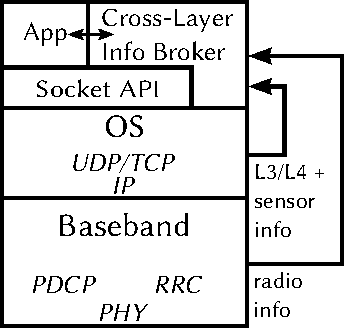
\includegraphics{images/cross-layer-model.pdf}
	\caption{Model and architecture of the proposed cross-layer information exchange.}
\label{c5:fig:crosslayer-model}
\end{figure}

Figure~\ref{c5:fig:crosslayer-model} illustrates the concept with the example of a mobile device. In a fully isolated model, no information would be passed from the baseband to the \gls{os} and the applications. The cross-layer model permits certain information to pass from one layer to another. Here, a software broker is responsible to collect information from several sources and layers and make it available to any interested application in a concise manner. 

This is an indirect cross-layer approach bypassing the intermediate layers completely and leaving them mostly unmodified. Also, information is always collected and used on the same device, making it purely vertical and distributed. Sharing this kind of information between different hosts would be accompanied by certain privacy and security implications due to potential data leakage. Most of the data is very sensitive and also be used with malicious intent.

This architecture is intended to pass data from the physical and link layer directly up to the application. Especially information specific to \gls{3G} mobile networks could be potentially interesting and used in benefit for applications and the user experience.This could include:

\begin{itemize}
	\item Information on the occurrence of a horizontal handover between cells.
	\item Information on neighboring cells and predictions when a handover is most probable to occur.
	\item Information on the prediction of the occurrence of a vertical handover and thereby changes in the active network stack, e.g., to the WiFi layers.
	\item Information on the current signal strength, bit error rate, and throughput.
	\item Detailed mobility information, including current location and travel speed in relation to base station positioning and availability.
\end{itemize}

Today, most of this information is only available inside the link layer or even just known to the mobile network's control plane. The impact of this ignorance can be significant for applications. For example, traffic scheduled during a handover period can be subject to especially high latency and loss due to the lengthy control plane interactions and traffic rerouting processes in a mobile network. If a cross-layer exchange would be provided and the application is made aware when an handover is supposed to occur, traffic could be schedule around the event. 

Generally speaking, the goal of the cross-layer approach would be to find meaningful reactions for every type of state the lower layers report through the broker. The pool of recipients is also not necessarily limited to certain applications. Especially the transport layer could be interested into explicit connectivity information and be modified to react accordingly. In addition to information flow, a path for control flow could also be envisioned. Herein, applications could directly influence the decision making and policies of the lower layers and adapt them to their personal needs.

All in all, the cross-layer data needs as well as the recipient's reactions need to be well defined and thoroughly tested to avoid any conflicts and layer separation issues. The impact of a simple unidirectional information flow on the layering mechanisms is suggested to be rather low. Only explicit and specific information is revealed keeping most of the isolation intact. However, a bidirectional control flow could soften up the isolation and have adverse side-effects. 

Either way, when implementing any kind of cross-layer exchange, one always has to keep a close look on the resulting consequences. One side effect can be the creation of an unintentional feedback loop between the control mechanisms of protocols of different layers. Moreover, breaches in the isolation could leak network state that could be exploited by malicious parties in any number of unforeseeable ways. Therefore, handling these plays an important role in cross-layer research. In \cite{1404568} some of these issues are presented and discussed.


\paragraph{Scenario: Reliable Streaming}

\gls{HTTP} traffic is especially suited to this scheduling behavior because of its statelessness and consistence of small objects that can be requested and transferred independently.

part 2: adaptive reliable streaming case

part 3: other beneficiary use cases: notifications in interactive communication

 E.g., \gls{TCP} retransmissions and congestion control could be adjusted in the course of understanding this.

% ! <-- !


\paragraph{Scenario: User Hinting}





%%





\begin{itemize}
	\item Video/Voice calls that notify the other party, that interruptions are expected to occur.

	\item Using current location data and movement patterns/predictions to improve cell selections and initiate horizontal and vertical handovers to a time suitable for the device and running applications.

	\begin{figure}[htb]
	        \centering
	        \begin{subfigure}[b]{0.90\textwidth}
	            \centering
				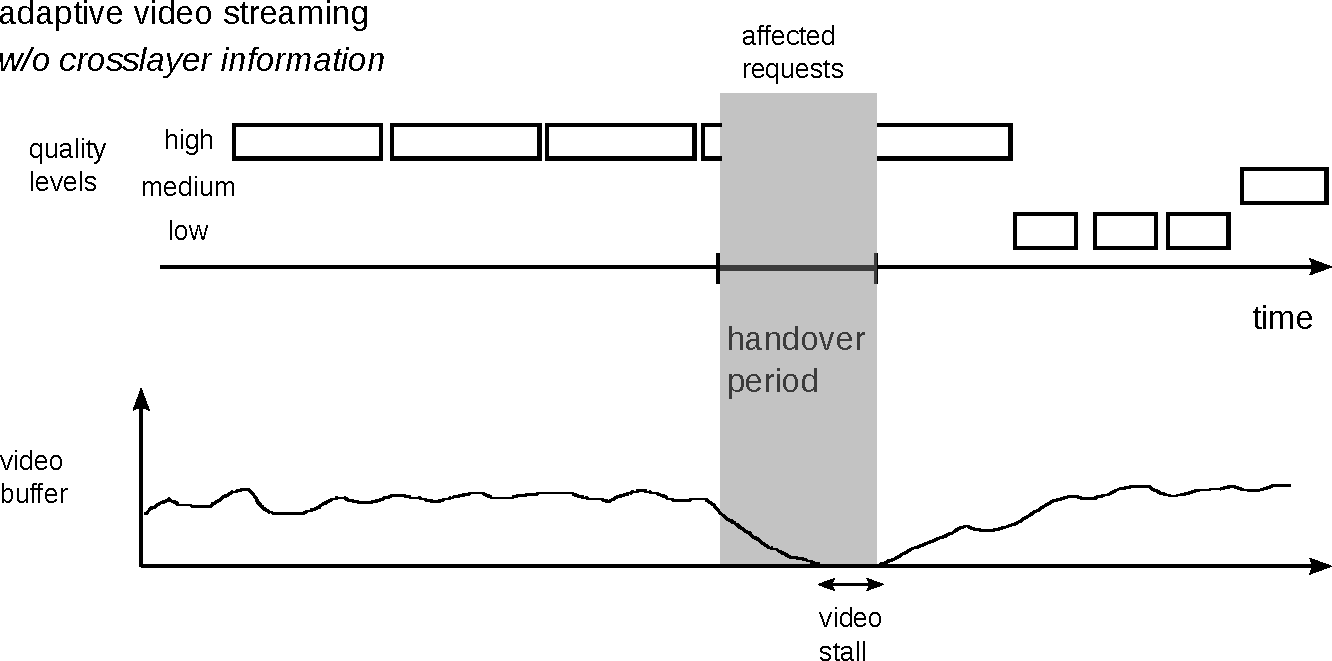
\includegraphics[width=\textwidth]{images/adaptive-streaming-no-cl.pdf}
				\caption{Stalling occurs without handover hinting.}
				\label{c5:fig:streaming-hinting-no-cl}
	        \end{subfigure}%

	        \begin{subfigure}[b]{0.90\textwidth}
				\centering
				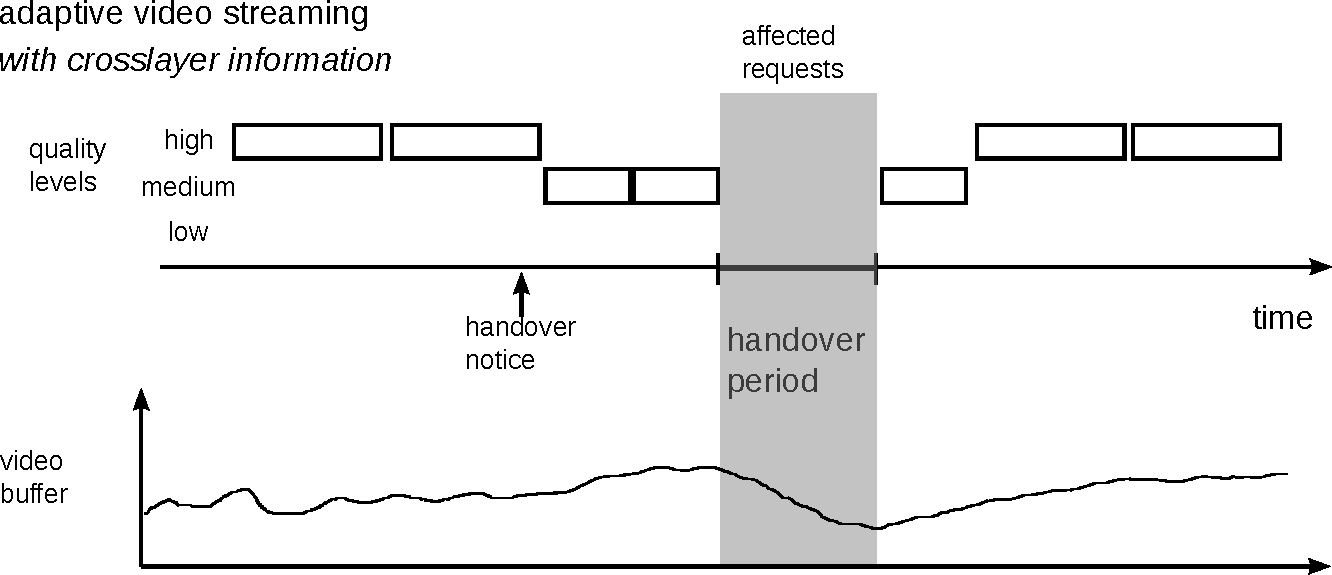
\includegraphics[width=\textwidth]{images/adaptive-streaming-cl.pdf}
				\caption{Stalling can be prevented by hinting and proactively filling the playback buffer.}
				\label{c5:fig:streaming-hinting-cl}
			   \end{subfigure}%
	 \caption{Mockup of handover prediction and hinting for adaptive streaming and thus avoiding playback stalls.}
	\label{c5:fig:streaming-hinting}
	\end{figure}

	\item An adaptive streaming video application increases its video buffer when a shortly upcoming handover is announced to survive the service outage. This can be achieved by an increased rate of segment retrieval and a reduction in segment quality. The goal is to avoid any possible playback stalls due to the handover. Figure~\ref{c5:fig:streaming-hinting} demonstrates this circumstance.

	The process:
		\begin{itemize}
		\item Tell Transport/Application the expected time till handover / time of uninterrupted service
		\item Tell Transport/App expected connection parameters (latency, BW, ...)
		\item Application selects \gls{DASH} stream appropriate to parameters
		\item Application reorders \gls{HTTP} GETs so that large GETs are not interrupted
		\item Application stops transfers when handover is about to occur
		\item Layer 1/2 gives a list of possible handovers to Application
		\item Application selects (better: suggests) handover which fits best and reorders accordingly
	\end{itemize}

	\begin{figure}[htb]
	        \centering
	        \begin{subfigure}[b]{0.90\textwidth}
	            \centering
				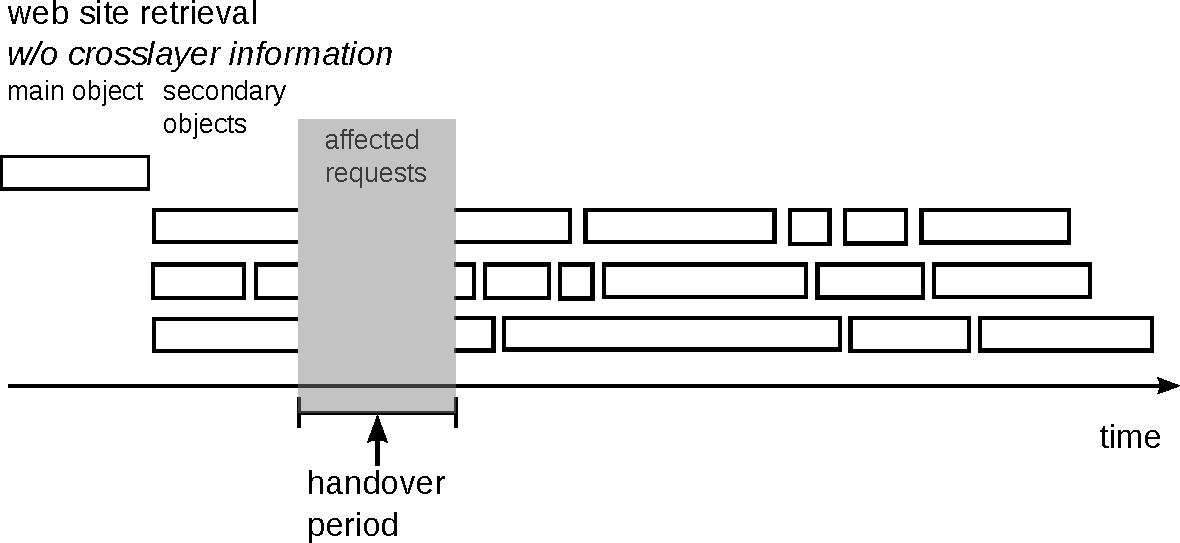
\includegraphics[width=\textwidth]{images/http-reorder-no-cl.pdf}
				\caption{The handover will block currently active object transmissions, page display will be delayed.}
				\label{c5:fig:http-reorder-no-cl}
	        \end{subfigure}%

	        \begin{subfigure}[b]{0.90\textwidth}
				\centering
				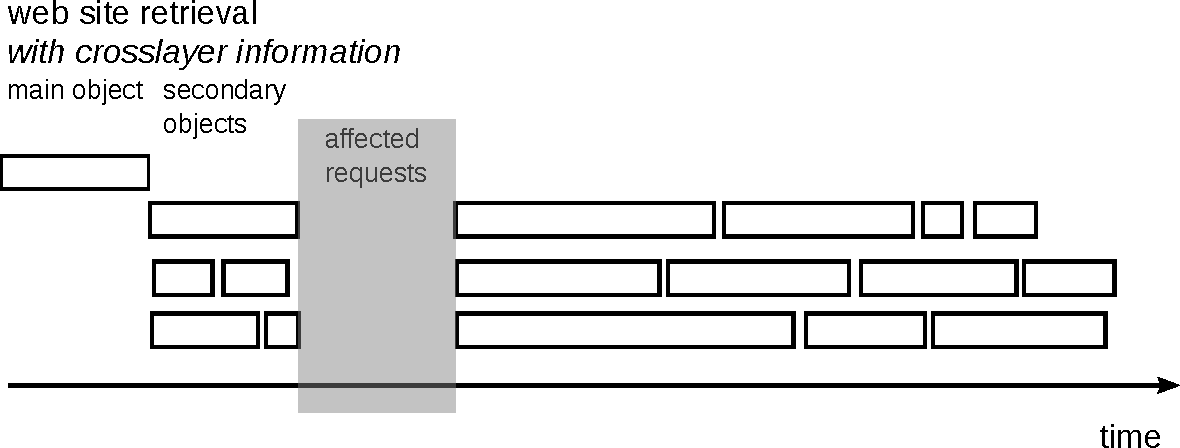
\includegraphics[width=\textwidth]{images/http-reorder-cl.pdf}
				\caption{The browser reorders the objects to be retrieved and avoids any transmissions during the indicated handover period.}
				\label{c5:fig:http-reorder-cl}
			   \end{subfigure}%
	 \caption{Mock-up of \gls{HTTP} reordering with handover awareness.}
	\label{c5:fig:http-reorder}
	\end{figure}

	\item Enable applications to adapt themselves to the conditions currently experienced by the networking stack and its sensors. For example, a Web browser could reorder its Website object requests to avoid sending any requests during handover periods and experience additional delay as seen in Figure~\ref{c5:fig:http-reorder}.

	\item A cross-layer enabled device can also offer a wide range of policy choices to its applications or even directly to the user. An example rule could be: ``Do not handover to a stationary WiFi from 3G when moving faster than 50km/h, only to in-vehicle WiFi.'' or ``Avoid any vertical handover, which would interrupt my service for a long time, while this VoIP call is running.''

\end{itemize}

Example Benefits

Put into relation:

\begin{itemize}
	\item frequency of handovers / distance/density of radio towers vs scenario traveling speed
	\item bit-length of streaming segments, typical transmission speed
	\item typical video length and number of segments
	\item derive number of interruptions in segments due to handovers
	\item estimate typical handover/mobility duration and service interruption time per event
	\item sum it up and compare to crosslayer information or even application layer handover decision
\end{itemize}






\begin{itemize}
	\item investigate how much information is exposed and what can already be done
	\item Analysis of data traces and realistic simulations in order to capture in detail the unwanted phenomena
	\item Verify the suitability of the State-of-the-Art algorithms and protocols which address this problem
\end{itemize}



\subsubsection{Implementation Approaches}

The Implementation:
\begin{itemize}
	\item Userspace daemon that collects information from kernelspace protocol implementations and sensors and provides them to all applications.
	\item shared bus control/information system, instead of explicit comm; signaling only to interested parties
	\item provide common interface also to all available sensors and layer 1 and 2 network information and control (similar to Android)
	\item IPC message bus, possibly D-Bus\footnote{\url{http://www.freedesktop.org/wiki/Software/dbus/}} based
	\item Could extend NetworkManager\footnote{\url{https://wiki.gnome.org/Projects/NetworkManager}}, some functionality is already provided there

\end{itemize}





%\subsubsection{Application Usage and Adaptation Scenarios}



% influence of signaling plane and core network elements - scaling
%This can apply to, e.g., reliability, frame sizing and fragmenting, and latency amounting to undesired effects on higher-layer traffic. 

 %Modem Link Properties Advertisement Protocol\footnote{\url{https://tools.ietf.org/html/draft-ivancic-mobopts-modemlpa-01}}

%LCP Link Control Protocol, PPP extension RFCs \cite{rfc1570,rfc1661}
%LISP and other mobility approaches \cite{rfc6830}

% Conceptually similar to cross-layer interactions is the family of dynamic radio resource management techniques. These control many properties concerning radio resources. 
% Radio Resource Management RRM
% 		\begin{itemize}
% 			\item resource monitoring, decision making, decision enforcement
% 			\item choose available wireless interfaces  best suited for a specific task
% 			\item rudimentary implementations in mobile OSs
% 		\end{itemize}
%	IEEE 802.21 cooperative handovers, but with required network support
%  Cross-layer design for wireless networks \cite{1235598} keine wirkliche aussage zu cross-layer

% User-centric mobility management for multimedia content access \cite{bolla2011usercentric} (not really cross-layer, uses something similar to LISP: an additional identifier shim and session migration for rtsp/sip) oddly mixed with user questionnaires

% Socketless \gls{TCP} --- an end to end handover solution \cite{1635680} % mobility scheme, not actually cross-layer information

%A ubiquitous mobile communication architecture for next-generation heterogeneous wireless systems \cite{1452832} (supposed to propose a function that determines the best handover initiation time in order to avoid early or late initiations)



	% - Research objectives
	% 	- Bidirectional vertical information and control flow on the performance of the individual layers
	% 		- Definition of generic interfaces
	% 		- Definition of a protocol (including information types, etc.)
	% 	- Definition of meaningful actions/reactions on the individual layers (e.g. adaptation of real-time communication data sources or changes in resource allocation)